%! Author = felix
%! Date = 17/03/2024

\renewcommand{\kapitelautor}{Autor: Felix Zwickelstorfer}
\subsection{Widgets}\label{sec:widgets}
\renewcommand{\kapitelautor}{Autor: Felix Zwickelstorfer}
Ein Widget beschreibt jedes Element, welches auf einem Screen sichtbar ist.
Die meisten werden von jedem Screen gebraucht, wie \zB das Box\-Widget, welches eine Flexbox darstellt, oder auch ein Bild oder ein Text.
Diese werden im folgenden als gewöhnliche Widgets bezeichnet.
Es gibt allerdings Elemente, die durch ihre Komplexität oder Dynamik nicht als eine Schachtelung von anderen Elementen dargestellt werden können.
Diese werden zu ihrem eigenen Widget, welches vom Controller verwaltet wird, wie \zB die Map.
\renewcommand{\kapitelautor}{Autor: Felix Zwickelstorfer}
\subsubsection{Widgets in Onj}\label{subsubsec:widgetsinonj}
\renewcommand{\kapitelautor}{Autor: Felix Zwickelstorfer}
Alle Widgets sind definiert in \inlineCode{assets/onjschemas/screen.onjschema}.
Als Beispiel folgt nun das grüne Icon in der Mitte:
\begin{codeBlock}{onj}{Beispiel: Definition eines Images aus heal\_or\_max\_screen.onj}
    $Image {
        name: "heal_icon",
        textureName: "map_node_heal",
        zIndex: 160,
        scaleX: 1.0,
        scaleY: 1.0,
        styles: [
            {
                positionType: positionType.absolute,
                positionTop: 19#percent,
                positionLeft: 47.15#percent,
            }
        ],
    }
\end{codeBlock}
Es gibt diverse Parameter, die nur für Images existieren, während andere "widget shared keys" sind, \dah, dass sie für alle gewöhnlichen Widgets verfügbar sind.
Diese beinhalten in dem oben angeführten Beispiel "name", "zIndex" und "styles".
Styles werden bei \ref{subsec:stylesystem} genauer beschrieben.
Es gibt allerdings auch die keys "behaviours" und "dragAndDrop", welche das Verhalten beim Interagieren des Benutzers definieren.

Ein Beispiel für ein spezielles Widget ist der Backpack:
\begin{codeBlock}{onj}{Beispiel: Backpack-Widget aus screens.onjschema}
    $Backpack {
        cardsFile: string,
        backpackFile: string,
        deckNameWidgetName: string,
        deckSelectionParentWidgetName: string,
        deckCardsWidgetName: string,
        backPackCardsWidgetName: string,
        backpackEditIndicationWidgetName: string,
        sortWidgetName: string,
        sortReverseWidgetName: string,
        ...widgetSharedKeys,
         children?: $Widget[],
         partOfSelectionHierarchy?: boolean,
    }
\end{codeBlock}
%    Wegen Ziel-H 2a Rucksacksystem
Der Rucksack ist eigentlich nur eine Box mit erweiterten Funktionen.
Man kann Kartendecks bauen, benennen und die Karten außerhalb des Decks, der sogenannten Kartenablage, nach gewissen Kriterien sortieren.
Dadurch, dass es ein eigenes Widget ist, kann und wird es auf mehreren Screen verwendet.
Es beinhaltet alle Keys, welche auf eine Box hat (alles ab den "widget shared keys"), und zusätzlich die Namen zu bestimmten Konfigurationsfile (cards und backpack), um die Daten richtig darzustellen.
Diese werden mitgegeben, da es eine schönere Lösung ist, als die Pfade hartkodiert im Code stehen zu haben.
Weiteres hat es noch und zusätzlich die Namen der bestimmter child-elemente.
Diese Elemente werden statt von dem Screen-controller, von dem Backpack Widget verwaltet oder verwendet.
%\begin{figure}[H]
%    \centering
%    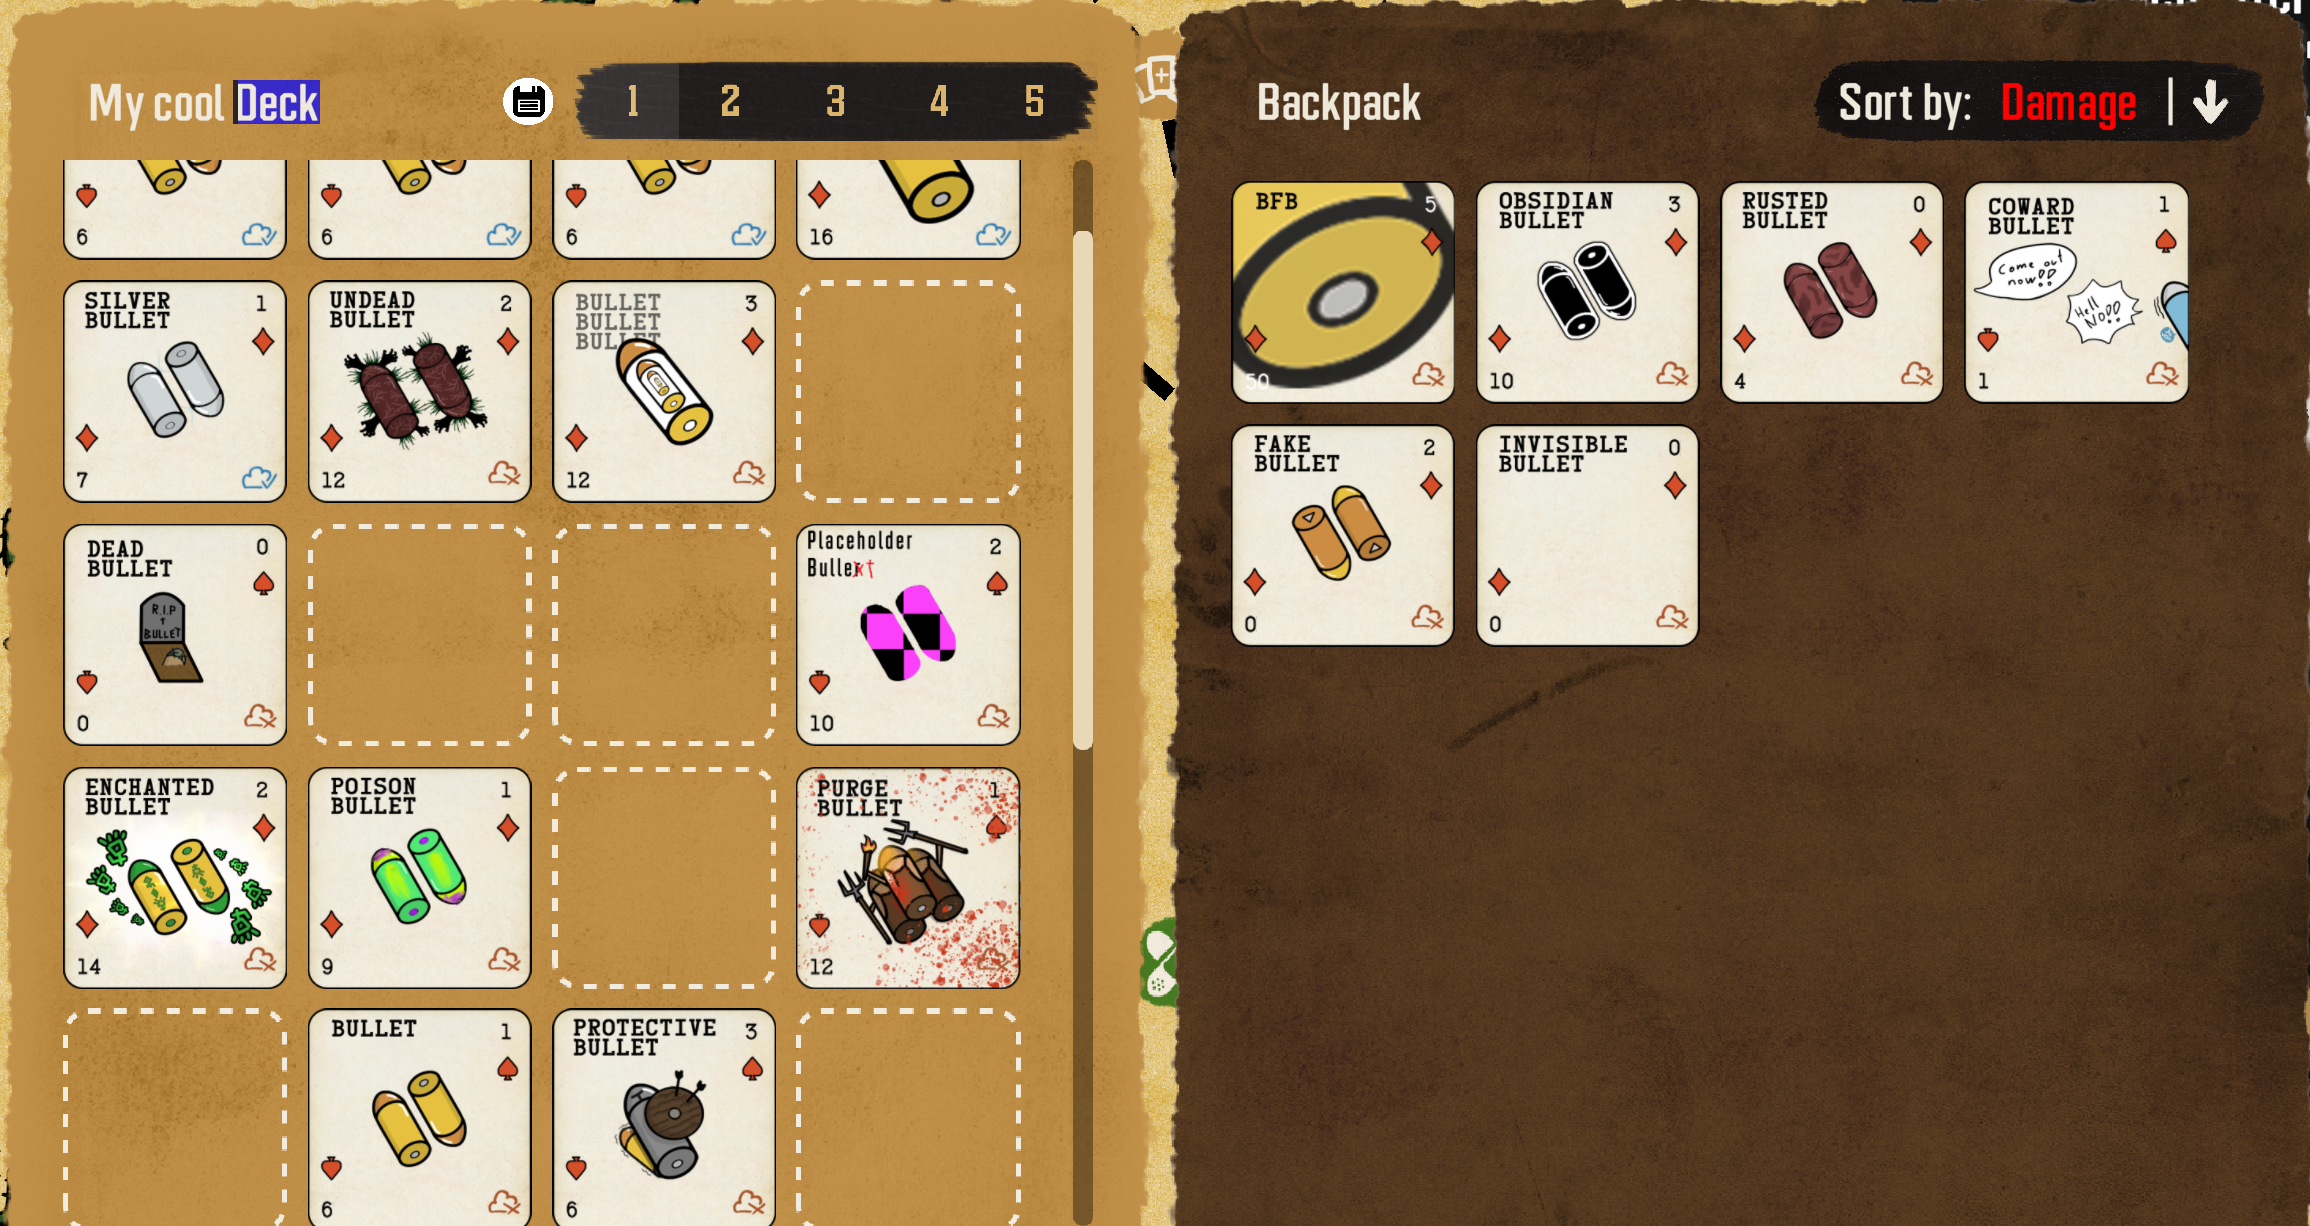
\includegraphics[width=1.0\textwidth]{backpack.png}
%    \caption{Beispiel: Screenshot des Backpacks}
%\end{figure}
\renewcommand{\kapitelautor}{Autor: Felix Zwickelstorfer}
\subsubsection{Widgets in Kotlin}\label{subsubsec:widgetsinkotlin}
\renewcommand{\kapitelautor}{Autor: Felix Zwickelstorfer}
Bei gdx ist ein Widget immer ein \inlineCode{com.badlogic.gdx.scenes.scene2d.Actor} oder eine Unterklasse davon.
In Forty-Five werden keine der Klassen von gdx direkt verwendet, sondern immer eigene Erweiterungen, wegen des Style-Systems wie bereits oben beschrieben.
Weiteres werden sie benötigt, um eigene Events verarbeiten zu können, wie das Hover-Event.
Programmtechnisch gibt es vier Hauptänderungen, die überschrieben werden:
\begin{enumerate}
    \item Die Layout Funktion, welche beschreibt, wo welche Elemente positioniert sind und bei Boxen auch deren Kinderelemente.
    \item Die Draw Funktion, welche für die Darstellung verantwortlich ist. Das ermöglicht es, Shader hinzuzufügen oder das Style-System einzubauen.
        Sie wird jeden Frame ein mal ausgeführt und wird daher ebenfalls zum updates von Timelines (siehe~\ref{subsec:timelines}) verwendet.
    \item Interfaces werden hinzugefügt, welche einerseits für das Style System verwendet werden, als auch generell das Arbeiten mit Widgets vereinfacht.
\end{enumerate}
\renewcommand{\kapitelautor}{Autor: Felix Zwickelstorfer}
\subsubsection{Templates}\label{sec:templates}
\renewcommand{\kapitelautor}{Autor: Felix Zwickelstorfer}
Templates sind ein weiterer wichtiger Part von Widgets, da sie das dynamische Erstellen von Elementen im Code erleichtern.
Außerdem verbessern sie die Lesbarkeit des Codes, da sehr ähnliche Widgets als ein Template mit mehreren Parametern definiert werden kann.
Alle gewöhnlichen Widgets können als Template erstellt werden.
Dies wird vor allem bei Karten verwendet, da das Design und das Verhalten innerhalb eines Screens für die Karten meistens gleich ist.
Deshalb erstellt man ein Widget aus einem Template und es wird nur das Bild und der Hover-Text auf die entsprechende Karte angepasst.
Templates werden allerdings auch an vielen anderen Stellen verwendet, \zB bei den Warnungen und Hinweisen im Backpack, als auch bei dem HealOrMaxHP-Screen für die beiden auswählbaren Widgets.
Ein templates zeichnet dadurch aus, dass es zusätzlich zu den normalen keys noch einen "template name" und die "template keys" hat.
Diese sehen bei dem Beispiel screen folgendermaßen aus:
\begin{codeBlock}{onj}{Beispiel: Ausschnitt eines Templates aus heal\_or\_max\_screen.onj}
templates: [
    $Box {
        template_name: "healOptionTemplate",
        template_keys: {
            "name": "name",
            "children.1.template": "templateMainText",
            "children.0.textureName": "textureName",
        },
        name: "Die name-value wird überschrieben, weil der zugehörige key in den templates angegeben ist",
        children: [
            $Image {
                textureName: "heal_or_max_add_max_health",
                scaleX: 0.8,
                scaleY: 0.8,
            },
            $TemplateLabel {
                template: "+5 Max HP",
                font: "red_wing_cm",
                color: color.dark_brown,
                fontScale: 1.1,
                align: "center",
            },
        ],
    }
]
\end{codeBlock}
Im Programmcode gibt man, wenn man ein template verwenden will, den template name an, und man gibt ein OnjObject mit, welche die zu überschreibenden Daten beinhaltet.
In diesem Beispiel sind es der angezeigte Text und das Bild, da diese sich von der linken und rechten Seite unterscheiden.
Weiteres wird über das template auch der interne Name des Widgets gesetzt.